\`E stato un ingegnere e matematico statunitense, \textbf{Claude Elwood Shannon} (1916 – 2001), che per primo ha
fatto diventare l’informazione qualcosa di ben definito e misurabile fornendo delle basi fondamentali per i
sistemi di comunicazioni.\\
Shannon ha lavorato nei laboratori Bell dal ’41 al ’72 e nel 1948 ha pubblicato “\href{http://www.math.harvard.edu/~ctm/home/text/others/shannon/entropy/entropy.pdf}{\emph{A Mathematical Theory of Communication}}” su The Bell System Technical Journal, una relazione tecnica che ora è alla base della Teoria dell’Informazione. \\
Oltre a definire e dare un’unità di misura all’informazione, la teoria di Shannon permette di rispondere anche a due domande fondamentali:
\begin{itemize}
    \item Quale è la massima compressione dei dati informativi senza perdita che si può ottenere.
    \item Quale è il massimo rate di trasmissione che si può avere per comunicazioni affidabili.
\end{itemize}
Gli studi di Shannon intendevano infatti migliorare l'efficienza della trasmissione dell’informazione: 

\textit{“Il problema fondamentale della comunicazione consiste nel riprodurre in un punto, esattamente o
approssimativamente, un messaggio selezionato in un altro punto.”}

L’importanza dei risultati degli studi di Shannon sta anche nel fatto che permettono di ridurre a forme
analitiche abbastanza semplici, problemi in realtà molto complessi e generali. \\
Dato un messaggio prodotto da una sorgente informativa, l’obiettivo della teoria dell’informazione è capire
come si deve rappresentare tale messaggio per ottenere una trasmissione efficiente dell’informazione in esso
contenuta su di un canale di comunicazione reale, ovvero soggetto a inevitabili limitazioni fisiche. \\
Questo obiettivo viene perseguito attraverso quattro passi fondamentali:
\begin{enumerate}
    \item \hyperref[sec:def]{Definizione e misura} dell’informazione di una sorgente.
    \item Capire, data una sorgente informativa, \textit{come} e \textit{quanto} è possibile ridurre il suo rate di trasmissione (\hyperref[sec:sorg]{\textit{Codifica di Sorgente}}).
    \item Definire cosa sia la capacità di comunicazione di un canale e sotto quali condizioni i dati provenienti da una sorgente informativa possono essere trasmessi in modo affidabile (\hyperref[sec:rdt]{\textit{Rate Distortion Theory}}).
    \item Come si può sfruttare al massimo la capacità di trasmissione di un canale rimuovendo (o rendendo trascurabili) gli effetti del canale di comunicazione (\hyperref[sec:can]{\textit{Codifica di Canale}}).
\end{enumerate}
\begin{figure}[H]
    \centering
    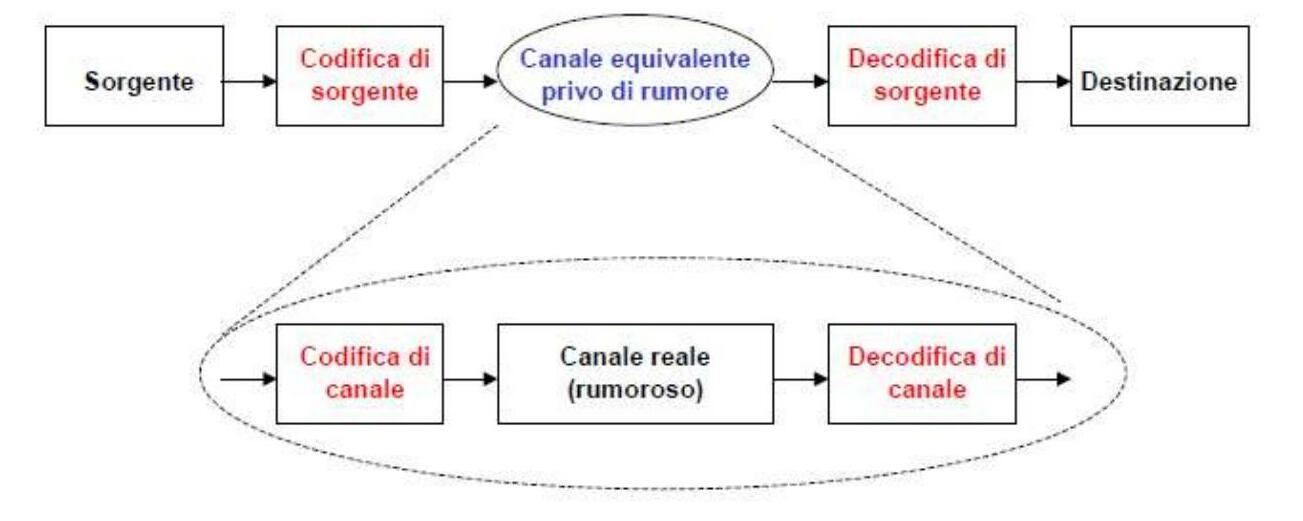
\includegraphics[scale=0.2]{img/croppedim.jpg}
    \caption{Percorso del messaggio, dalla sorgente al destinatario.}
    \label{fig:percorso}
\end{figure}
Come raffigurato in Figura \ref{fig:percorso} la codifica (sia di sorgente che di canale) si deve adattare alla sorgente e al canale in modo da avere la massima efficienza possibile nel trasferimento dell'informazione:
\begin{itemize}
    \item La \textit{codifica di sorgente} adatta la sorgente alla trasmissione su di un opportuno canale equivalente privo di rumore.
    \item La \textit{codifica di canale} permette di trasmettere l’informazione emessa dalla sorgente (opportunamente
trattata mediante la codifica di sorgente) in maniera affidabile su un canale reale caratterizzato da limitazioni fisiche.
\end{itemize}

\begin{center}
  $\ast$~$\ast$~$\ast$
\end{center}

Questi appunti sono stati elaborati principalmente sulla base del materiale pubblicato dal titolare del corso, a cui vanno tutti i crediti. I riferimenti principali oltre a questo sono stati:
\begin{enumerate}
    \item \textit{\href{https://www.wiley.com/en-it/Elements+of+Information+Theory,+2nd+Edition-p-9780471241959}{Elements of Information Theory} - Thomas M. Cover \& Joy A. Thomas.}
    \item \textit{\href{http://clem.dii.unisi.it/~vipp/files/TIC/dispense.pdf}{Lecture notes on Information Theory and Coding} - Mauro Barni \& Benedetta Tondi.}
    \item \textit{\href{http://www.inference.org.uk/mackay/itprnn/book.html}{Information Theory, Pattern Recognition, and Neural Networks} - David MacKay.}
\end{enumerate}
Chiunque volesse contribuire a questo materiale, segnalando degli errori o estendendo il contenuto, mi pu\`o contattare a \href{mailto:gio.bindi@pm.me}{gio.bindi@pm.me}.
\begin{flushright}
Novembre 2019.
\end{flushright}